
\documentclass[11pt]{article} % use larger type; default would be 10pt

\usepackage[utf8]{inputenc} % set input encoding (not needed with XeLaTeX)

%%% PAGE DIMENSIONS
\usepackage{geometry} % to change the page dimensions
\geometry{a4paper} % or letterpaper (US) or a5paper or....
\geometry{margin=1in} % for example, change the margins to 2 inches all round
% \geometry{landscape} % set up the page for landscape
%   read geometry.pdf for detailed page layout information

\usepackage{graphicx} % support the \includegraphics command and options

% \usepackage[parfill]{parskip} % Activate to begin paragraphs with an empty line rather than an indent

%%% PACKAGES
\usepackage{booktabs} % for much better looking tables
\usepackage{array} % for better arrays (eg matrices) in maths
\usepackage{paralist} % very flexible & customisable lists (eg. enumerate/itemize, etc.)
\usepackage{verbatim} % adds environment for commenting out blocks of text & for better verbatim
\usepackage{subfig} % make it possible to include more than one captioned figure/table in a single float
% These packages are all incorporated in the memoir class to one degree or another...

%%% HEADERS & FOOTERS
\usepackage{fancyhdr} % This should be set AFTER setting up the page geometry
\pagestyle{fancy} % options: empty , plain , fancy
\renewcommand{\headrulewidth}{0pt} % customise the layout...
\lhead{CS 5150 Final Report}\chead{}\rhead{Sun in the City Group}
\lfoot{}\cfoot{\thepage}\rfoot{}

%%% SECTION TITLE APPEARANCE
\usepackage{sectsty}
\allsectionsfont{\sffamily\mdseries\upshape} % (See the fntguide.pdf for font help)
% (This matches ConTeXt defaults)

%%% ToC (table of contents) APPEARANCE
\usepackage[nottoc,notlof,notlot]{tocbibind} % Put the bibliography in the ToC
\usepackage[titles,subfigure]{tocloft} % Alter the style of the Table of Contents
\renewcommand{\cftsecfont}{\rmfamily\mdseries\upshape}
\renewcommand{\cftsecpagefont}{\rmfamily\mdseries\upshape} % No bold!

%%% END Article customizations

%%% The "real" document content comes below...

\title{CS 5150 Final Report \\ Sun in the City Group}
\author{Phillip Tischler (pmt43), Brian Toth (bdt25), Vera Khovanskaya (vdk9), \\ 
Sean Salmon (ss2669), Lin Xue (lx39), Zach Porges (zip2),  \\
and James McGuinness (jrm369)}
%\date{} % Activate to display a given date or no date (if empty),
         % otherwise the current date is printed 

\begin{document}
\maketitle


\begin{figure}[h!]
\begin{center}
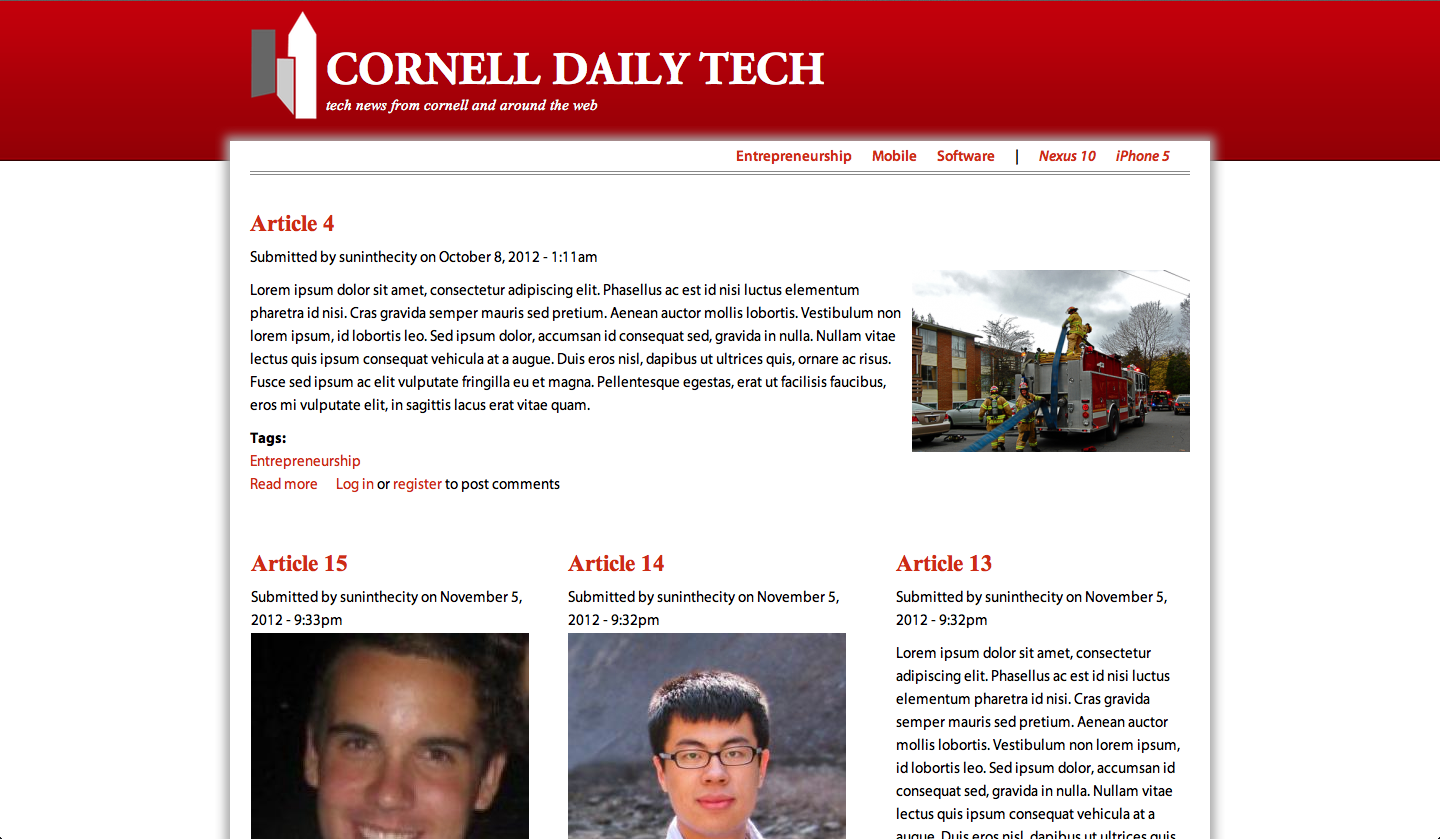
\includegraphics[width=\columnwidth]{images/homepage}
\end{center}
\caption{The Homepage of The Cornell Daily Tech}
\end{figure}

\clearpage
\tableofcontents
\clearpage

%%%%%%%%%%%%%%%%%%%%%%%%%%%%%%%%%%%%%%%%%%%%%%%%%%%%%%%%%%%%%%%%%%%%%%%%%%%%%%%%
\section{Project Description}

The goal of the project is to create a new website and Content Management System (CMS) for the Cornell Daily Sun for a new market: Cornell’s new Tech Campus in New York City. According to the client, Joseph Staehle, IT Manager for the Daily Sun, it should be a ``Totally online, totally tech based newspaper for the tech campus.”

The website is being built using Drupal, but will involve a custom front-end design as well as intelligent back-end technology. The website will include data fusion, or the aggregation of articles from other news sources.

%%%%%%%%%%%%%%%%%%%%%%%%%%%%%%%%%%%%%%%%%%%%
\subsection{The Team (Skills, Experience, and Contribution)}

The team has a diverse background of technical knowledge as well as leadership and project experience. It has been determined that the backgrounds are more than sufficient to tackle this project. All members have familiarized themselves with the core technologies of the project prior to the feasibility study in order to talk intelligently about the topic. That is, each member has become familiar with HTML, CSS, PHP, MySQL, setting up a web server (Apache web with PHP and MySQL), and setting up Drupal. Each member was responsible for specific parts of the project and handled all aspects of that component. That is, each member designed each component, developed each component, documented each component, and tested each component they were responsible for.

\textbf{Phillip Tischler (pmt43@cornell.edu)}. Phillip is currently the Team Lead of an engineering project team at Cornell (CUAir, Cornell University’s Unmanned Air Systems Team) which includes managing development of 36 engineers. Previous to this position he was the Software Sub-team Lead and managed 8 software developers. His relevant experience in industry is when he lead development of a team of two other full time employees to create web software to manage large scale database and data processing engines, of which the software was deployed internally to approximately 100 operations employees. Phillip is responsible for project management, system design, database development, shared library development, and for deployment.

\textbf{Brian Toth (bdt25@cornell.edu)}. Brian has programmed in Java, C, C\#, and Clojure. He has worked with Linux, Windows, and Git. His relevant experience includes developing an image-processing plugin for a large commercial software platform, and creating data acquisition software for an off-road racing vehicle for an engineering project team at Cornell (Cornell Baja SAE). His notable CS coursework includes 5414 (Distributed Computing), 5412 (Cloud Computing), 5430 (System Security), 5780 (Machine Learning), and 5620 (Intro Computer Graphics). He is currently a TA for CS 4410/4411 (Operating Systems). Brian shares the responsibility of developing the Data Fusion backend system. 

\textbf{Vera Khovanskaya (vdk9@cornell.edu)}. Vera is an expert at visual prototyping software, Adobe Photoshop, Adobe Fireworks, and Adobe Illustrator. She has been researching Human-Computer Interaction for 2.5 years and has extensive experience with usability testing, role-play, and case analysis. In this research she has deployed and tested mobile health software, conducted open-ended interviews, and done design and prototyping work. In addition, she is fluent with HTML, CSS, and PHP. Vera is responsible for designing the front end, performing use case analysis, and performing user testing and validation. 

\textbf{Zach Porges (zip2@cornell.edu)}. Zach is our team’s expert in HTML, CSS, PHP, MySQL, and mobile application design. He has developed web applications for the Ithaca Innovation Firm, a student run web and logo design firm. He is currently the TA for INFO 1300 (Intro to Design and Programming for the Web) and INFO 2300 (Intermediate Design and Programming for the Web). Zach is responsible for the HTML, CSS, and other components related to the front end display of the website.

\textbf{Sean Salmon (ss2669@cornell.edu)}. Sean has extensive experience with Java programming, HTML, constraint modeling, and statistical data analysis. He has completed CS 1110 and CS 2110. Currently Sean is working on CURB Website Design and has obtained experience with DreamWeaver and CSS. Sean is responsible for developing the custom Drupal modules that are used to display and edit Data Fusion information.

\textbf{Lin Xue (lx39@cornell.edu)}. Lin is an experienced programmer with Java, Python, and C. He also has skills in Adobe Photoshop, Adobe Illustrator, Google SketchUp, and AutoCAD. In addition, he is also proficient in data analysis and is familiar with Mathematica and Origin. Lin has researched for over 4 years and has obtained experience with experimental physics in nanoscale magnetic devices, he has designed data acquisition software (LabWindows) as well as data analysis software (Python). He has published journal papers and given conference presentations. Lin shares the responsibility of developing the Data Fusion backend system.

\textbf{James McGuinness (jrm369@cornell.edu)}. James is proficient with Java, C, C++, OCaml, and Python. He’s worked with the Windows API and has experience via a variety of small projects done out of interest, as well as larger scale projects from CS 3110 and CS 3410. He also has some experience with statistical aggregation from previous projects. James is responsible for the RSS Parsers that feeds data from other sources into the Data Fusion backend system.

%%%%%%%%%%%%%%%%%%%%%%%%%%%%%%%%%%%%%%%%%%%%
\subsection{The Client}

The client for this project is The Cornell Daily Sun, a for-profit organization with its operations being run independently from Cornell since 1880. Currently the Cornell Daily Sun is the main source of news on campus regarding issues related directly to Cornell University students. The organization has both a print newspaper and an online newspaper, and generates revenue with the placement of advertisements. The points of contact in The Cornell Daily Sun are IT Manager Joseph Staehle, and Editor in Chief Juan Forrer.  Mr. Staehle presented the proposal and will be the primary client and point of contact for this project.

\begin{figure}[h]
\begin{center}
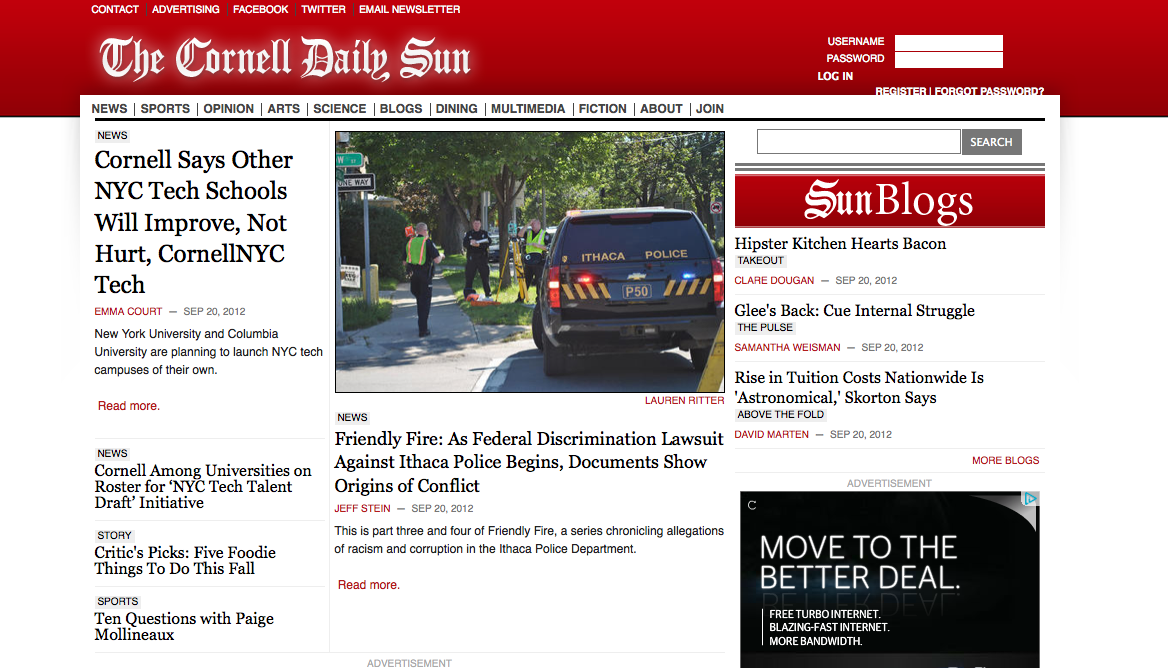
\includegraphics[width=\columnwidth]{images/cornell_sun_current}
\end{center}
\caption{The Cornell Daily Sun's Current Website}
\end{figure}

\subsubsection{Availability}

In regards to availability, Mr. Staehle is a student at Cornell University and resides on campus, and thus his schedule aligns with that of our teams which makes scheduling client-group meetings simple. Additionally, The Cornell Daily Sun is located in the Commons of Ithaca which is a short walk from Cornell campus. The team has met numerous times outside of milestone meetings. Thus the client has been available.

\subsubsection{Concerns}

The client has demonstrated to the team the commitment to seeing this project through its development and deployment. However, two concerns were raised during various meetings. The success of the project post deployment relies on generating content writers as well as readers of the website, a task that can only be solved by the client. This raises two issues. First, The Cornell Daily Sun does not currently have writers for the proposed project. Secondly, generating a critical mass of website readers may be more difficult than expected. On a quarterly basis, The Cornell Daily Sun’s current website has approximately 80,000 unique visitors. This newspaper caters to the Cornell student population, a user base of approximately 13,000 undergraduates and 2,000 graduates. The difference in number of visitors is likely due to a vast pool of alumni that also read the website. The project proposed is one for the new Cornell Tech Campus, a campus that does not yet have an alumni populus to bridge the gap in number of readers. This concern has been voiced to the client, and steps to mitigate the issues are being taken. That is, The Cornell Daily Sun is now in the process of recruiting writers and determining how long it would take to obtain the critical mass of readers.

The second concern involves the deployment to AWS (Amazon Web Services). The client has had trouble obtaining access and funding for the service. The team is evaluating the option to deploy temporarily on their own funds in order to demonstrate deployment. Either way, the team will deploy to a virtual machine and record the process via screencast. This will be part of the handover documents that the client will receive, which will allow the client to deploy on a different timescale.

%%%%%%%%%%%%%%%%%%%%%%%%%%%%%%%%%%%%%%%%%%%%
\subsection{Scope \& Requirements}

The project analyzed in this document is one to build a new website and Content Management System (CMS) for The Cornell Daily Sun. This website will represent a new market for the client. That is, the client is attempting to expand its newspaper to begin bringing news to the students of Cornell University’s new Tech Campus in New York City.
                   
\subsubsection{System Status}
                   
The Cornell Daily Sun website is an existing product that is managed with a Drupal CMS and custom extensions. This project is to build a new website for the Cornell Tech Campus, and is therefore a new product and not an augmentation or replacement. However, if this new website is extremely successful the old website may be converted to the new one. To maintain familiarity with the CMS system, the client has requested the CMS be based on the Drupal CMS.

\subsubsection{Actors and their Use Cases}

\textbf{Reader}. Readers are the consumers of both the primary and secondary content on the website. They will generate the bulk of traffic to the system as there are orders of magnitude more readers as other types of actors. The use case they will primarily exercise is that of reading content on the website. They can find this content by either searching for it or browsing the various categories. It will be important to build trust with these users so that they desire to engage with the main content and with the secondary sources that we hope to integrate. Our own experiences with news content align most closely with this use-case, so we hope to accomplish preliminary usability testing on ourselves; however, as we grow more accustomed to the interface as developers, it will become increasingly important to test this use case on external audiences. This use case is of primary interest as it will define the success or failure of our client as these external stakeholders will generate the revenue.

\textbf{Editor}. This is that actor that represents our clients, and is of high priority because they will have the most responsibilities and most investment when interacting with the system. Editors exercise the use cases of editing content posted by writers, determining which content should be posted to the website, and approving the Data Fusion sources. Editors are the executors of the newspaper’s broader vision, and the intermediaries between the writers and the users. Editors will also need to understand how to maintain the system, and will be particularly sensitive to the various data fusion and machine learning algorithms the team may be implementing. It is important to consider the editors' needs in usability testing because they are the "keystone species" of this news content ecology.

\textbf{Writer}. The writers are the actors that generate primary content for the website and then decides what kind of secondary data, like Data Fusion sources, to include in their specific contribution. The use cases that writers go through are important to test because these actors are likely to be the less familiar with the system as they are least invested with The Cornell Daily Sun, and yet the most tech-savvy of our three actors as they will be generating content for a newspaper that is technical in nature.


\begin{figure}[h]
\begin{center}
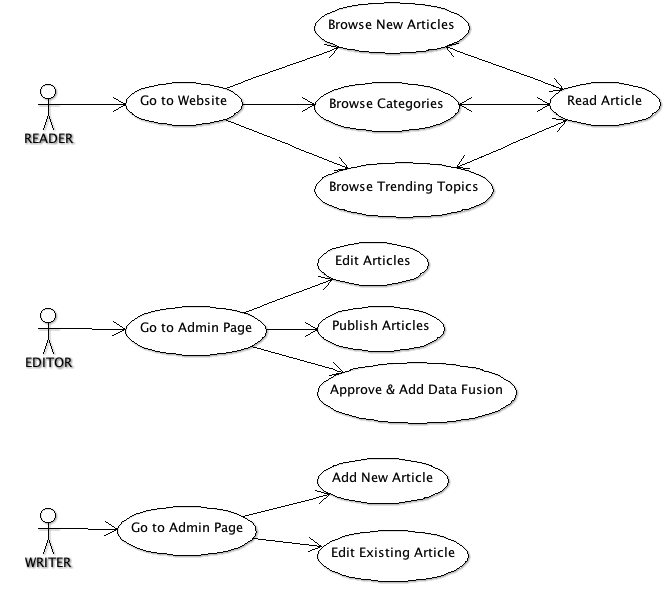
\includegraphics[width=4in]{images/use_case}
\end{center}
\caption{The Use Cases}
\end{figure}
                   
\subsubsection{Functionality}
                   
There are four required pieces of functionality the project must support: a website for readers to browse the newspaper, a CMS to manage the website and allow writers to post content, a means to allow Data Fusion to present external content inline with content generated by The Cornell Daily Sun, and finally a Brand to associate with this new website. Like the existing CMS The Cornell Daily Sun uses, the CMS must allow the writers and editors to upload their content like articles, blogs, comments, images, and advertisements. The website itself must display this content in a reasonable and convenient way that allows readers to browse and obtain the information they are looking for. To create a unique Cornell Tech campus newspaper, the project also requires the team to create a Brand. This includes a logo, a display name, and a look and feel for this newspaper. A key aspect of this Brand will be Data Fusion, a distinction from the current website the client operates. Data Fusion will present articles from external sources inline with an article posted by the Cornell Daily Sun. It is similar to a ``Read More" link, except this information will be external and automatically presented with the article from The Cornell Daily Sun.
                   
There are three desired but not required pieces of functionality for the project: an optimized mobile version of the site, an algorithm to perform the Data Fusion automatically, and a performance optimizer for the entire system. The mobile optimized site will allow readers to browse The Cornell Daily Sun’s website on a mobile device in a much faster and convenient way than to load the main page onto a slower device with less screen display area. This functionality may require too much time to implement, which is why it is not a required portion of this project. The Data Fusion described in the paragraph above was a framework to allow custom algorithms to link external content as well as manually link content. The other piece of functionality that is not required is an algorithm to automatically detect and link external content to the content generated by The Cornell Daily Sun. This may involve web and RSS feed scraping as well as Machine Learning and other advanced topics. Due to the complexity of the functionality relative to the timeframe of the project, this functionality has been deemed not required. However, if implemented it will save time, make running the website easier, and increase the attractiveness to potential readers as it will dynamically update the site. The final desired but optional piece of functionality is a performance optimization that will decrease the time it takes to load the website. Using a 50Mbps connection (an average user only has access to a 2Mbps connection), the client’s current site takes over 5 seconds to load the visible page of the homepage and over 13 seconds to load the entire page. Most websites can respond in under 200 milliseconds and load completely in a second. Every millisecond the user waits has a psychological impact on their perception of the website, and thus it is critical to load as fast as possible. There are simple upgrades to the system that can be employed to achieve this goal. However, time and budget may be a limiting factor, which is why this functionality is desired but not required.

\subsubsection{Technical Requirements}

The technical requirements of the project are to host a web server, create a website that loads quickly, construct the system with the Drupal 7 CMS system, and be designed well enough to allow the system to be maintained by the IT managers of The Cornell Daily Sun. The website will be hosted on Amazon AWS as per the request of the clients. This will provide a standard hosting environment, regional server provisioning, automatic server scaling, and elastic load balancing at no additional price other than time to configure. The current website owned by The Cornell Daily Sun, when uncached by the user, takes approximately 5 seconds to load the visible part of the homepage and more than 13 seconds to load the homepage completely on a 50Mbps connection. It is desired to have each page respond in about 200 milliseconds and finish loading in about two second on a typical network connection (10Mbps). We know this to be possible as the current website contains about 1.6MB of data on a page, and on a 10Mbps network would take 1.28 seconds plus about 40 milliseconds in network latency. Additionally, to achieve this will require regional server partitioning, use of an elastic load balancer, use of soft state cache servers, and then finally the main content generation server. This is the route the team will take if the team has time to tackle the desired but not required functionality and if the clients have the funds to deploy such a system. The system must be built with the Drupal 7 CMS as the users of the site need to be familiar with the operation of the CMS. As The Cornell Daily Sun’s current site runs with Drupal, it will be an easy transition. Finally, the system design must be modular and well documented so that it can be maintained by IT managers of The Cornell Daily Sun.

\subsubsection{Scale Estimates}

The new website that will be developed is expected to achieve the same scale once it is fully adopted. This includes 20,900 page requests per day (648,000 in the last month), at least 3GB of memory to handle requests at peak load, over 170,000 unique users per month, 4GB worth of static data, and 2.8 GB of data in a MySQL database.

\subsubsection{Dependencies}

\textbf{Drupal}. Drupal is an open-source CMS that The Cornell Daily Sun uses for their current website, and as such the CMS that will be used for this project. The Drupal CMS is licensed under the GNU General Public License. This license is explained under the discussion of business considerations. Drupal is composed PHP, HTML, and CSS to generate and display the content, and a MySQL database to store the information composing the content itself. Drupal 6 requires PHP 4.4.0 or higher, while Drupal 7, the latest release, will be used and it requires PHP 5.2.5. Drupal provides a large baseline of features for a website, including but not limited to, user account handling, layout management, website menu customization, RSS feed aggregation, article search, and FTP access. Extensions can be written for Drupal in PHP, and there are over 17,000 free extensions available that are also under the GNU General Public License. For this project, Drupal will provide a very strong base for building this system.

\textbf{Deployment Server}. We will be using a Linux-based server hosted on a cloud platform for purposes of development and eventually deployment. The plan is to use Amazon AWS as the cloud provider. Because Drupal uses PHP and MySQL only, a Linux server is appropriate.

\textbf{Data Fusion}. The Data Fusion extension is integrated into Drupal using a PHP module, but the core functionality of the scraper will be written in Java. Because Drupal already has RSS aggregation, it is very likely that the module will rely on some form of RSS news scraping to find similar news articles.

\textbf{Apache Lucene}. The Data Fusion algorithm will be using the Apache Lucene indexing and search library that is licensed under the Apache 2.0 license. This license has been vetted and determined appropriate for this project.
                    
\subsubsection{Business Considerations}

Drupal is licensed under the GNU General Public License, so we are able to download, reuse, modify, and distribute any files from Drupal’s Git repositories. The Daily Sun already uses Drupal, so we do not foresee any licensing issues involving their new website. More details are available here: http://drupal.org/licensing/faq/. The copyright to all code that we write for this project will be owned by the Daily Sun.

We do not anticipate any major problems, but a few potential risks involve acquiring enough readers and writers. Currently, The Cornell Daily Sun’s website reaches about 80,000 unique visitors per quarter. It will take time to build up a large audience for the tech campus’ website, as there will be very few students, and no alumni. The Sun will also need a strong editorial team to write the news and this team has not yet been hired. Finally, the Sun’s IT managers will need to set up and maintain hosting for the new website. The Cornell Daily Sun hopes for this site to be profitable in the long-run. They do not yet have specific targets, but they will need to bring in enough revenue from ads to exceed their costs.

We do not anticipate the need to maintain any technological trade secrets or patents at this time. If such topics arise they will be dealt with in an appropriate manner.

Our team believes that the level of complexity for this project is very appropriate. Most of the code for the CMS is already written, and we will be able to scale the complexity of our data fusion element based what our team is able to accomplish. The project is extremely unlikely to fail, but even if it does, this would not be a huge problem for The Cornell Daily Sun as it will not hurt its current business.

%%%%%%%%%%%%%%%%%%%%%%%%%%%%%%%%%%%%%%%%%%%%
\subsection{Benefits}

There are two unique stakeholder entities that will benefit this project. The first is The Cornell Daily Sun that will own the product that results from the project. The second is the students and other community members of Cornell University’s new Tech Campus. Each entity will benefit in different ways from the success of this project.
                   
\subsubsection{Cornell Daily Sun}
                   
With the new website, The Cornell Daily Sun will both expand its market, increase its influence, and increase its revenue. This project will allow the client to new types of content for both its paper based and web based publications. As the website matures, the project will allow the client to attract new readers on the order of 80,000. As the website displays advertisements, there will be a new source of income for the Cornell Daily Sun. Finally, with the new content and new readers in the New York City area, the website is very likely to attract new advertisers.
                   
Another potential benefit of the project is the integration of new technology. That is, the current website the client runs is on an older Drupal 6 CMS whereas the new website will be built with Drupal 7. Our new design will better organize the website content, and eciency code will be used to improve the compiling time from minutes to seconds. The Drupal 7 has major improvements over the Drupal 6. They are enhanced security (for scheduled tasks, password, and log-in), usability (better support for both administrators and users), and performance (new features for search, file handling, and RSS feeds). These new technical improvements are desired in the current Cornell Daily Sun website. If this project is a success, it can be deployed to replace the current website as well.
                   
\subsubsection{The Cornell Tech Campus Community}
                   
The website to be developed provides a way for broadcasting current news about the Cornell NYC Tech campus, which serves the Tech campus members and the general Cornell community. With blog services in addition to news, the website also enables individuals to share information with the community about tech topics, their life, campus life, alumni activity, and career experience. 

%%%%%%%%%%%%%%%%%%%%%%%%%%%%%%%%%%%%%%%%%%%%%%%%%%%%%%%%%%%%%%%%%%%%%%%%%%%%%%%%
\section{Project Design}

%%%%%%%%%%%%%%%%%%%%%%%%%%%%%%%%%%%%%%%%%%%%
\subsection{User Interface Design}

After examining a set of 16 top tech news blogs and identifying common themes, design strategies, and resulting implications, we developed a design vocabulary that described each website in the “space” we studied as a series of tradeoffs that were expressed in a website’s design.
                
Our first tradeoff was “Designing for editorial control vs. popularity” which is most visible in the difference between aggregate news blogs (sorted by popularity) and editorially controlled websites (such as the new york times.) The advantage of leaning toward popularity is that it is easier to maintain the site, but exercising editorial control may be more in line with the branding and corporate image.
                
The second tradeoff we identified was the tradeoff of content; while this was not a primary focus for us, we noticed that different sources appealed to different audiences: some websites were directed at people with significant pre-existing technical knowledge while others were aimed toward mainstream readers (with few assumptions about their existing knowledge). We decided that our content should appeal to “hardcore nerds,” but also to the general “tech curious” public.
                
Our final trade-off was between dynamic vs. static data organization; some of the websites that we reviewed had several, nested menus that reflect various aspects of technical news. We felt as though these tended to get cumbersome as technical fields changed, and decided that the best way to handle this trade-off would be to allow some categories to be permanent, while others are temporary and change with trending topics. We will have permanent links on the homepage that filter articles by categories including news and entrepreneurship, but other links that can easily be modified by editors with trending tags.
            
Using the trade-offs that we described, our interface emphasizes editorial control over popularity, focuses on a broad audience with an emphasis on Tech campus student interests, and includes both static and dynamic elements in the navigation.
            
Our client outlined a relationship between our website and their main Cornell Daily Sun brand; our website incorporates aspects of the original brand such as the general website layout, color scheme, and page layout structure. We deviated from the main brand in aspects that are specific to the Cornell Daily Tech. Obvious examples of the stylistic deviation include a different logo (because we have a different name), and a different article presentation: larger images, but linear, “blog style” presentation to accommodate slower content addition. 

%%%%%%%%%%%%%%%%%%%%%%%%%%%%%%%%%%%%%%%%%%%%
\subsection{System Design}

The system has been designed to be as modular and uncoupled as possible. The Cornell Daily Sun’s current website is highly coupled and has prevented them from upgrading their system form Drupal 6 to Drupal 7.

The website will be hosted on Amazon AWS running an Apache 2 Web Server and a MySQL Database Server. Drupal 7 will be used to provided the base CMS and website structure. The team will develop custom XHTML, CSS, and PHP to create a ``theme" in Drupal. This customization can easily be ported to other Drupal versions and is a lightweight display layer. This will generate the viewable site and handle HTTP requests.

\begin{figure}[htbp]
\begin{center}
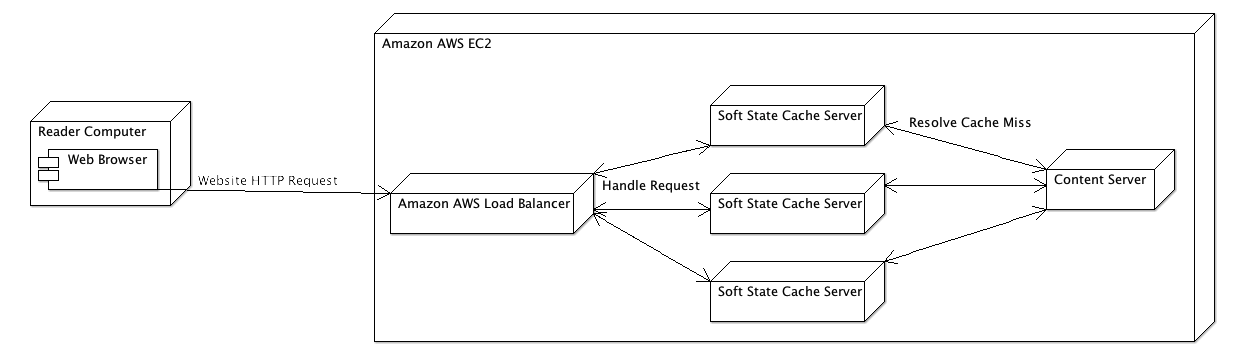
\includegraphics[width=\columnwidth]{images/data_flow}
\caption{Deployment Diagram}
\end{center}
\end{figure}

A Varnish server will be used as a soft-state in memory cache server. It works as a reverse proxy HTTP server and can handle about 3,000 page requests a second. This will provide incredible performance and scalability of the new site. Drupal also has pre existing modules to integrate with Varnish. This allows Drupal to invalidate page cache entries as the website is updated by The Cornell Daily Sun and happens completely behind the scenes.

Java will be used for the Data Fusion algorithm. The first component is RSS and Website Feed scraping. Various libraries are being analyzed to handle this workload. Essentially, the program will listen to RSS feeds and store the data in a MySQL database. Another component, the indexer, will take the data that has been scraped and put it into an Apache Lucene Index. Finally another component, the data fusion algorithm, will use the meta-tag taxonomy of an article to search for relevant data in the RSS and Website Apache Lucene Index, and store likely matches in another MySQL table.

To choose which Data Fusion articles get posted on the website, the team will build a lightweight PHP Drupal Extension to allow editors to approve fusion results as well as add in manual fusion data. This module will be an extremely lightweight and as decoupled as possible.

\begin{figure}[htbp]
\begin{center}
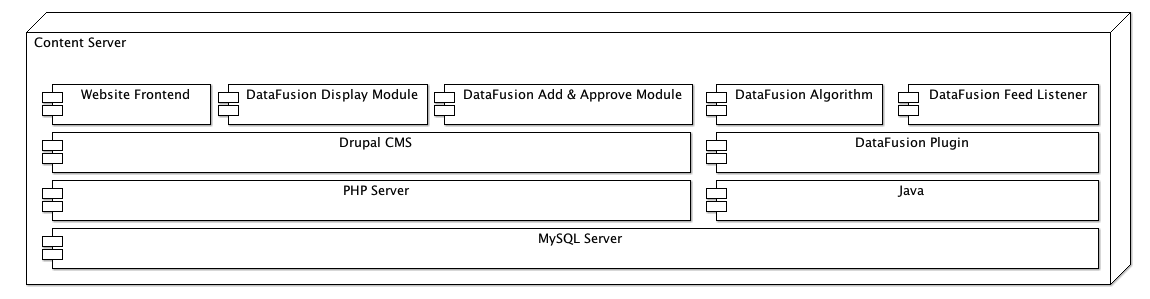
\includegraphics[width=\columnwidth]{images/software_stack}
\caption{System Architecture}
\end{center}
\end{figure}

%%%%%%%%%%%%%%%%%%%%%%%%%%%%%%%%%%%%%%%%%%%%
\subsection{Code Design}

\subsubsection{Website Interface}

Implementation of the interface involved a combination of modifying CSS, installing third-party modules, and modifying Drupal settings. CSS was modified in the sun sub-theme, which overrides CSS from Zen, a simple theme that makes it easy to create sub-themes.

\subsubsection{Database Design}

The database was redesigned to the new schema shown below. In the diagram you can see the DataSource table which represents a source of information like The New York Times. Any source can have multiple DataMeans, which represent the generator of source content like The New York Times RSS Feed. These DataMeans objects then generate content which is represented in DataStored. The Data Fusion algorithm then takes various DataStored objects and creates DataFusion objects representing the logical link between external content and content written by The Cornell Daily Sun. The content by The Cornell Daily Sun is represented by a node, which is the article representation in Drupal.

\begin{figure}[htbp]
\begin{center}
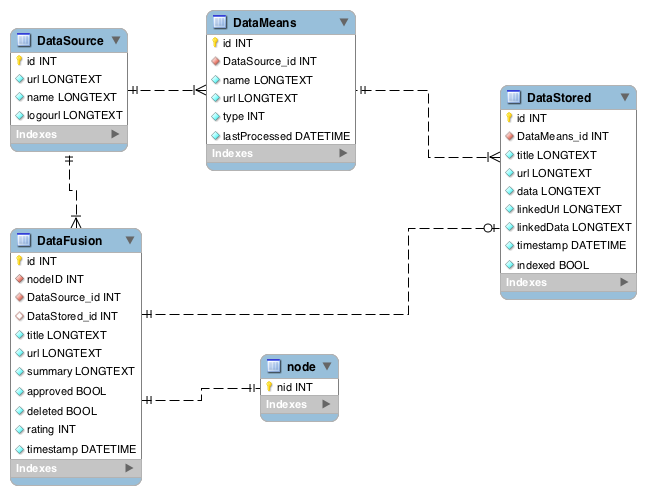
\includegraphics[width=\columnwidth]{images/database_schema}
\caption{Database Schema}
\end{center}
\end{figure}

\subsubsection{Drupal Modules}

The Data Fusion drupal module is written primarily in PHP with small occurrences of CSS and HTML for formatting display of the results found by the Data Fusion algorithm. The module consists of 4 core files, ‘datafusion.info’,  ‘datafusion.module’, ‘datafusion.node.inc’ and ‘datafusion.admin.inc’.

Datafusion.info is the standard project description file containing information regarding the configuration version, package and core.

Datafusion.module is the header file for the module itself, containing several overiden default Drupal hook methods handling the view loaded on each page. In here lies many of the customizations the user might want to change given their preferences on permissions handling and authorization issues.

Datafusion.node.inc is one of the implementation files included in the project.  This file is a view handler for the page rendered after selecting the “Data Fusion” node tab. Within the confines of this file is both a connection to the MySQL database established and subsequent PHP queries of the database enacted. This file allows the user to add/edit/approve/reject auto-generated Data Fusion results from the database to be viewed alongside their article.

Datafusion.admin.inc is the other implementation file included in the project that handles the view for the page rendered under the Admin>Configuration menu. This is the view that gives the editor full reign over the Data Fusion articles, Data Sources and Data Means existing on the website while allowing them to add and edit in their own articles/sources/means as well.

\subsubsection{Shared Library}

TODO PHILL

\subsubsection{RSS Parser}

The RSS Parser is written in Java, utilizing some external libraries- specifically, ROME, JDOM, Log4J, and the sun.datafusion.data libraries. The purpose of these libraries is to provide an efficient method of reading external XML pages (JDOM) such that ROME may present the list of posts in a quick, efficient manner. Log4J is used for logging purposes.

There are two main classes in the RSS Parser- RSSParser and RSSGrabber. The prior is designed to connect to a MySQL table using the Manager class in sun.datafusion.data and iterate over all entries in the database’s DataMeans table, while the latter is used by RSSParser to grab articles for DataMeans objects given by Manager.getDataMeansToProcess(). The RSSParser, after grabbing articles, writes these back to the MySQL table using the same Manager object. Timestamps are updated and written to the database to ensure duplicate posts aren’t written back to the database on later calls to RSSParser.parse().

\subsubsection{Data Fusion}

TODO Brian \& Lin

%%%%%%%%%%%%%%%%%%%%%%%%%%%%%%%%%%%%%%%%%%%%
\subsection{Testing}

\subsubsection{Website Interface}

The website was built on Drupal’s CMS, which has already been tested extensively. Manual testing was performed by viewing/adding/deleting articles, menu links, comments, and other content that users would access.

\subsubsection{Drupal Modules}

In order to properly test the functionality of the module, several manual testing procedures were performed. Apart from code that manages front end operations, testing of the back end consisted of multiple queries of the database. These tests were enacted through physical input into the text fields for adding and editing articles, data sources, and data means as well as selecting choices from the option wheel. Expected results from queries (updating, adding and deleting), were found to be true in the database. 

\subsubsection{Shared Library}

The shared library was written in Java to abstract at a logical level the representation of data. That is, each entry in the MySQL table is modeled as a Java object. The other algorithms interact with the MySQL database through a Manager class that represents the logical operations that would be desired, like get all DataStored objects that need to be indexed. In this way, the logical operations are completely decoupled so that improvements to queries, data storage, and other components can be implemented without affecting the operation of other components.

\subsubsection{RSS Parser}

Due to the nature of the different classes within the RSS parser, testing will be examined for each class separately.

First, the RSSGrabber class must be tested in order to ensure the RSSParser class functionality (if this class breaks, RSSParser breaks as well). To do so, a unit test has been created and provided in RSSUnitTest.java. This includes a main method, and test three RSS feeds to make sure they are being retrieved correctly. Due to the nature of how RSSGrabber works, the main (and probably only) issue will arise when connecting and getting the RSS posts through ROME; one that is complete, it’s just a simple matter of a Java iterator (guaranteed to work) and some getters and setters (also, guaranteed to work due to their simplicity). It will print any errors along with “Unit test complete” when it is finished.

The function grabHTML in RSSGrabber was only manually tested with RSSParser. This is due to the volatile and simple nature of the function; either grabHTML can open a HTTP connection and get a string, or it can’t and throws an IOException.

RSSParser runs a very simple process, using mostly external classes for a complex functionality. Due to this, a failure in one of the classes it uses (specifically the Manager and RSSGrabber classes) will cause RSSParser to fail or not behave correctly. Because of this, manual testing to ensure that the process RSSParser works is sufficient. This can be simply done by either using the provided Main.java file in the parser package, or by creating MySQL entries in a database for the parser to read, and a table for it to write to (make sure to create the tables correctly and set the properties file to ensure the Manager class looks at the right tables).

Self-done manual tests showed that the RSSParser process worked without issue, and any bugs or problems that arose originated from any classes it was using to complete its process. The only internal logic in RSSParser is a simple Java iterator loop, which is guaranteed to function by the Java API.

\subsubsection{Data Fusion}

TODO Brian \& Lin

%%%%%%%%%%%%%%%%%%%%%%%%%%%%%%%%%%%%%%%%%%%%%%%%%%%%%%%%%%%%%%%%%%%%%%%%%%%%%%%%
\section{Validation}

%%%%%%%%%%%%%%%%%%%%%%%%%%%%%%%%%%%%%%%%%%%%
\subsection{User Validation}

To validate our interface’s usability, we employed a series of user test methodologies. Ideally, we would have done a full user test with tests who are a representative sample of all our “actors” outlined earlier in the document, but due to time constraints, we experimented with discount methods for some of the actors. Our primary concern was meeting the needs of the content writers, and to validate that our software is user-friendly, we did a simple user-test with a current Cornell Daily Sun blog writer. We were fortunate to have a test who primarily works on generating “blog” content. We asked our test user to edit an existing article, view and approve data-fusion options, and add a new source to the data fusion list. Client Validation was fully successful for the first two tasks, but we had to prompt our user to find the interface to add websites to the data fusion table. From this, we learned that our training module should focus on good technical specifications for this task. Our discount methods for the other actors were cognitive walk throughs in which we critically assessed tasks that editors and readers would do in using our interface. For editors, this involved changing articles and data fusion, and closely resembled tasks that we did in our user test. For the viewers, we walked through task such as reading the homepage, navigating to a subsection, and searching for an article. It is not clear that these cognitive walkthroughs yielded novel results for our interface development, but we used the critical awareness to refine our design and compare our interface to analogous websites in the same domain (New York Times, Bits, and Cornell Daily Sun) to validate stylistically againsts the design paradigms in those websites. We thought it would be reasonable to cross-validate our interface against these others since users have internalized these design paradigms and would reasonably expect our website to act in accordance to them. In conclusion, we validated our interface in a user test which suggested that our interface was clear (exempting a global data fusion task) and we employed discount usability methods to validate our website against existing design models.

%%%%%%%%%%%%%%%%%%%%%%%%%%%%%%%%%%%%%%%%%%%%
\subsection{Client Validation}

Our primary form of validation was meeting with the client and making sure that they were satisfied with our product. Our client validation consisted of a lengthy and meticulous meeting, in which we presented all aspects of the website and asked the client whether it satisfied his requirements. During this meeting, we primarily made design changes. Namely, we implemented a different grid on the home page, changed the number of rows in the navigation (two row, one for permanent, one for trending) and moved the search box. At the conclusion of the client validation meeting, our client signed off on our project and stated that he was satisfied with the product. 

%%%%%%%%%%%%%%%%%%%%%%%%%%%%%%%%%%%%%%%%%%%%%%%%%%%%%%%%%%%%%%%%%%%%%%%%%%%%%%%%
\section{Documentation}

%%%%%%%%%%%%%%%%%%%%%%%%%%%%%%%%%%%%%%%%%%%%
\subsection{JavaDoc}

TODO Brian

%%%%%%%%%%%%%%%%%%%%%%%%%%%%%%%%%%%%%%%%%%%%
\subsection{Code Walkthrough}

\subsubsection{Website Interface}

The website is built using Drupal, so interface elements were built and can be modified using Drupal’s GUI. The following third-party modules are used for the interface:

\begin{itemize}
\item Nodes in Block - Featured article on homepage
\item Pathauto - Improved URLS for SEO
\item Special Menu Items - Add non-URL text in menu
\item Views, Views UI - Grid of articles on the homepage
\item Chaos Tools \& Tokens - Required by various modules
\item Adsense - Google ads
\item Display Suite - Modify teasers (article previews) on front page
\end{itemize}

Custom CSS was written in the Sun sub-theme, which is built on top of Zen, a simple template theme. Relevant CSS files are in the following directory: sites-\textgreater all-\textgreater themes-\textgreater sun-\textgreater css.
Relevant CSS files:

\begin{itemize}
\item pages.css - contains most of the custom formatting/styling
\item layouts->fixed-width.css - sets the width of the 2 columns (for all pages except the front page)
\item normalize.css – base styling
\item forms.css – forms
\item navigation.css – includes the menus with tags towards the top of the website
\end{itemize}

\subsubsection{Drupal Modules}

TODO Sean

\subsubsection{RSS Parser}

RSSParser is the basic object needed to parse from RSS feeds. It requires four fields- dbname, username, password, and server\_ip, all of which can be obtained through the Properties object given by PropertyUtils.loadProperties() from the sun.datafusion.utils package. These are used to establish a connection to the MySQL database using a Manager object (located in sun.datafusion.data).

Once initialized, calling RSSParser.parse() will retrieve all articles from the MySQL table, aggregate new RSS posts from them, and write those new posts back to the database, using the tables specified above. The parse() function starts by grabbing every DataMeans object in the MySQL database by using the function getDataMeansToProcess located in the Manager class. It then iterates over each of them (using a simple Java Iterator), creating a RSSGrabber object for each, which uses the function RSSGrabber.getNewPosts() in order to retrieve the new RSS articles in DataStored format. It then calls Manager.setDataMeansProcessed() to update the timestamp on the RSS feed to prevent duplicate posts on later iterations over that DataMeans object. Finally, it uses the same Manager object as before to write each of these DataStored object back to the database.

RSSGrabber is used by the RSSParser loop to actually parse the RSS feed. The object initially opens a connection to the feed URL in the DataMeans object passed to it via three object- first, a HTTPConnection object to the URL, then a XmlReader object (part of the JDOM library) and finally, a SyndFeed object (part of the ROME library). The SyndFeed object is built using the SyndFeedInput class from ROME; calling SyndFeedInput.build(XmlParser) will create the SyndFeed object. Upon calling getNewPosts() on the RSSGrabber object, it iterates through every RSS post in the RSS feed (presented via the SyndFeed object) and pulls the relevant data detailed above, storing it into a new DataStored object. If a field cannot be retrieved from the post, a null value is written. As part of this process, a URL connection to the URL linked in the RSS feed is opened in a method called grabHTML, spoofing as Firefox to ensure successful retrieval. It uses a BufferedReader object to do so, which is built from an InputStreamReader object from the URL connection. grabHTML returns a string value of the entire HTML source of the webpage, or null if it could not connect to the page.

If a RSS post has a date older than that of the lastProcessed timestamp on the DataMeans object, a DataStored object is not created for that post.

The RSS Parsing program writes INFO statements when it starts and finishes a parsing loop, and ERROR statement when there is an error in a specific DataMeans entry, recording the id of the entry that triggered the error. The logger name should be “sun.datafusion.parser.RSSParser” (sans quotation marks). This is set to INFO by default.

\subsubsection{Data Fusion}

TODO Brian \& Lin

%%%%%%%%%%%%%%%%%%%%%%%%%%%%%%%%%%%%%%%%%%%%
\subsection{User Training}

\begin{itemize}
\itemindent 0pt
\item Add an article
	\begin{itemize}
	\itemindent 10pt
	\item Admin->content->Add content
	\item Click “Article”
	\item Enter the title, body, tags, and image
	\item Ensure that the image width is at least 620 pixels
	\item Save
	\end{itemize}
\item Swap featured article
	\begin{itemize}
	\itemindent 10pt
	\item Add new featured article
		\begin{itemize}
		\itemindent 20pt
		\item Administration->content
		\item Click edit next to the name of the new featured article
		\item Towards the bottom, click “Nodes in block”
		\item In the select region dropdown, click Nodes in block 1 (Pos)
		\item Under visibility, enter “<front>”
		\item Save
		\end{itemize}
	\item Remove old featured article
		\begin{itemize}
		\itemindent 20pt
		\item Administration->content
		\item Click edit next to the name of the old featured article
		\item Towards the bottom, click “Nodes in block”
		\item In the select region dropdown, click None
		\item Save
		\end{itemize}
	\end{itemize}
\item Add permanent tag link to menu
	\begin{itemize}
	\itemindent 10pt
	\item Administration->Structure->Menus
	\item Click Add Link next to Main Menu
	\item In “Menu link title” enter the name of the tag
	\item In path, enter “tags/[nameoftag]”. For example, “tags/software”
	\item Save
	\end{itemize}
\item Add trending tag link to menu
	\begin{itemize}
	\itemindent 10pt
	\item Administration->Structure->Menus
	\item Click add link next to Trending Tags
	\item In “Menu link title” enter the name of the tag
	\item In path, enter “tags/[nameoftag]”. For example, “tags/3DS”
	\item Save
	\end{itemize}
\item Add a link to the “Information” list in the footer
	\begin{itemize}
	\itemindent 10pt
	\item Administration->Structure->Menus
	\item Click add link next to Footer information links
	\item In “Menu link title” enter the name of the page
	\item In path, enter a relative url (ex. “content/about”) or an absolute url (ex. “https://www.facebook.com/cornellsun”)
	\item Save
	\end{itemize}
\end{itemize}

%%%%%%%%%%%%%%%%%%%%%%%%%%%%%%%%%%%%%%%%%%%%
\subsection{Useful Links}

\begin{itemize}
\item https://help.ubuntu.com/community/ApacheMySQLPHP
\item http://drupal.org/documentation
\item http://lucene.apache.org/core/4\_0\_0/index.html
\item https://www.varnish-cache.org/docs
\item http://lucene.apache.org/core/
\item http://www.ibm.com/developerworks/opensource/library/os-apache-lucenesearch/
\item http://www.lucenetutorial.com/advanced-topics/scoring.html
\end{itemize}

%%%%%%%%%%%%%%%%%%%%%%%%%%%%%%%%%%%%%%%%%%%%%%%%%%%%%%%%%%%%%%%%%%%%%%%%%%%%%%%%
\section{Project Handover}

TODO

%%%%%%%%%%%%%%%%%%%%%%%%%%%%%%%%%%%%%%%%%%%%
\subsection{Development Setup}

TODO

%%%%%%%%%%%%%%%%%%%%%%%%%%%%%%%%%%%%%%%%%%%%
\subsection{Deployment}

TODO

%%%%%%%%%%%%%%%%%%%%%%%%%%%%%%%%%%%%%%%%%%%%
\subsection{USB Flash Drive}

TODO

\end{document}
